\section{Channel Saliency}\label{sec:ch4:occlusion}
To get another heuristic on the importance of the ScatterNet channels, let us examine
the effect on inference scores observed when zeroing out Scattering channels.
\cite{zeiler_visualizing_2014, zhou_object_2014} have done similar studies but
over patches of the input image, with the former using a patch of grey values as
the occlusion mask, and the latter using a set of random pixels. 

We must be careful to occlude with a sensible mask, the $S_0x$, $S_1x$ and $S_2x$
all have very different probability densities. Assuming $x \sim \mathcal{N}(0, \sigma^2I)$ 
(already a fairly weak assumption),
the pdf of $S_0x$ will also be a zero mean gaussian. However, the distributions
of $S_1x$ and $S_2x$ are more complex - the real and imaginary parts of the
$\DTCWT$ are sparse but are strongly correlated in energy. Further, after the modulus operation,
there is a strong positive bias to all the pdfs until the signal passes through
another bandpass filter. Choosing a sensible random mask is
therefore difficult, so we instead use a constant mask. Analysis of the
datasets show that zero is very close to the maximum likelihood value for each
channel so we occlude channels by simply setting them to zero at every spatial
location.

\subsection{Experiment Setup}
We take a network similar to the one from
\autoref{tab:ch3:scat_arch} but using the colour operation described in 
\autoref{sec:ch4:colour} so the scattering output has 51 output channels. We further
choose to set $C=50$ so the conv1 layer has 100 channels, a nice width to
display. We train this network
on the same 3 datasets - CIFAR-10, CIFAR-100 and Tiny ImageNet, and report the
drop in classification scores on the validation set after removing one channel at
a time. 

We additionally display the weight matrix for the first learned layer of the
network trained on Tiny ImageNet. This gives us a second perspective on the
channel importance by looking at the relative weights of the ScatterNet channels
passed on to the successive 100 channels. The weight matrix is convolutional
filter of size $w \in \reals[100\x 51\x 3\x 3]$. We define:
\begin{equation}\label{eq:ch4:arms}
  A^{rms}_{c, f} = \sqrt{ \frac{\sum_{i,j} w[f, c, i, j]^2}{{\sum_f \sum_{i,j} w[f, c, i, j]^2}} }
\end{equation}
This gives us a matrix $A^{rms}$ (for root mean squared) which has columns of
unit energy representing the different output channels after conv1. The row
values then show how much each scattering channel contributes to each output
channel. This is shown in \autoref{fig:ch4:weights}.

\subsection{Discussion}
First we look at Tiny ImageNet in \autoref{fig:ch4:occlusion1}.
Note that when any of the $S_0$ channels are removed, 
the validation accuracy drops sharply for all 3 datasets. A similar result
happens when any of the $S_1$ channels are zeroed out. 

For both the first and second scales of the first order coefficients, 
$S_1^1$ and $S_1^2$, there are two channels that seem less
important - the second and fifth channels, corresponding to the $45\degs$ and
$135\degs$ wavelets. Often the high-high portion of the first scale coefficients
are considered mostly noise, but this does not explain why the $45\degs$
and $135\degs$ channels for the second scale coefficients are also less
important. A possible interesting conclusion to be drawn from this is that the
dataset does not have as many diagonal edges in it as horizontal and vertical
edges. 

To test this, we retrain the network but this time rotate the input
images randomly $30\degs$ clockwise or anti-clockwise in both training and
validation. We then rerun the occlusion experiment for all channels and plot the
resulting changes in \autoref{fig:ch4:ti_rotated_occlusion}. Interestingly, for
this network, the $45\degs$ and $135\degs$ wavelets for $S_1^2$ are now the most
important of the 6, which validates our assumption. The corresponding wavelets
for $S_1^1$ have become more important, but it is likely that they remain less
salient because of the effects of the higher bandwidth for the diagonal
wavelets.

Comparatively, the $S_2$ channels have little effect on the classification score
when individually masked. The four largest drops in accuracy for
$S_2$ happen when $\theta_1 = \theta_2 \in \{15\degs, 75\degs, 105\degs, 165\degs\}$.
When $\theta_1 \neq \theta_2$ we saw the ripple like patterns in
\autoref{fig:ch4:reconstructions}, and we see here that the network has mostly
learned to not depend on them.

\autoref{fig:ch4:weights} tells a similar tale for the Scattering channels. Here
we see directly how much and how little each of the channels is used by the
first layer of the network, with the low intensity values in $S_2$ indicating that the
next layer's outputs are less dependent on these coefficients.

We include the same analysis for the two CIFAR datasets in
\autoref{fig:ch4:cifar_occlusion} for completeness, although the insight gained
here is the same - the $S_2$ coefficients are the least important. One notable difference to
\autoref{fig:ch4:occlusion1} is in the $S_1^2$ coefficients, which have reduced importance 
in CIFAR, but with the smaller input spatial size, this comes as no surprise.

\begin{figure}
  \vspace{0cm}
  \centering
  \subfloat[Tiny ImageNet]{\vspace{-1cm}
    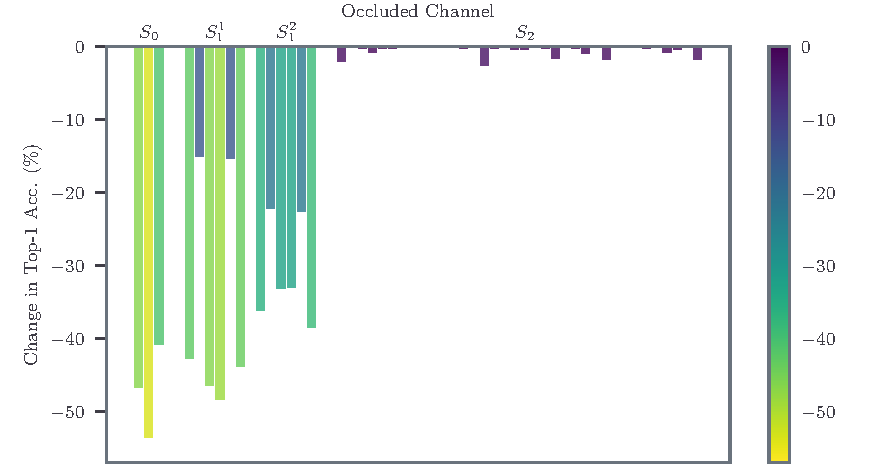
\includegraphics[width=15cm,height=8cm]{\imgpath/ti_occlusion_colour.pdf}
    \label{fig:ch4:ti_occlusion}
    }
    \\
  \subfloat[Rotated Tiny ImageNet]{
    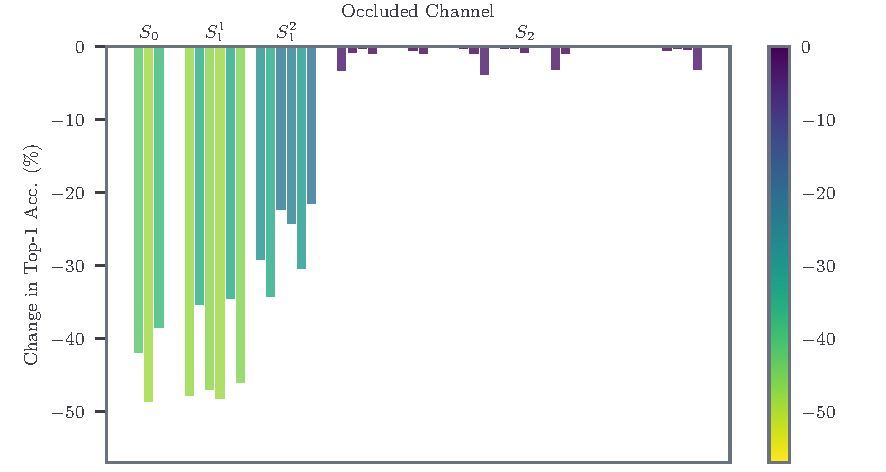
\includegraphics[width=15cm,height=8cm]{\imgpath/ti_rotated_occlusion_colour.pdf}
    \label{fig:ch4:ti_rotated_occlusion}
    }\vspace{-0.3cm}
  \mycaption{Tiny ImageNet changes in accuracy from channel occlusion}{Numbers
  reported are the drop in final classification accuracy when a channel is set
  to zero. The bars are coloured relative to their magnitude to aid seeing the
  differences for the $S_1$ coefficients. \subref{fig:ch4:ti_occlusion} When 
  any of the lowpass channels $S_0$ are removed, the classification accuracy
  drops sharply, note that the middle channel, corresponding to green, is
  unsurprisingly the most important of the three colours. The first scale, first
  order scattering coefficients $S_1^1$ are slightly more important than the
  second scale coefficients. The 36 $S_2$ coefficients
  have very little individual effect on the validation score when removed.
  \subref{fig:ch4:ti_rotated_occlusion} The same network trained with input
  samples rotated by $\pm 30\degs$. In \subref{fig:ch4:ti_occlusion} 
  the second and fifth orientations for both $S_1^1$ and $S_1^2$,
  corresponding to the $45\degs$ and $135\degs$ wavelets,
  are comparatively less important than other orientations at the same scale.
  This suggests that perhaps the dataset does not have much diagonal
  information. When rotated this trend changes and the diagonal
  wavelets at both scales become more important.}
  \label{fig:ch4:occlusion1}
\end{figure}

\begin{figure}
  \centering
  \hspace{-1cm}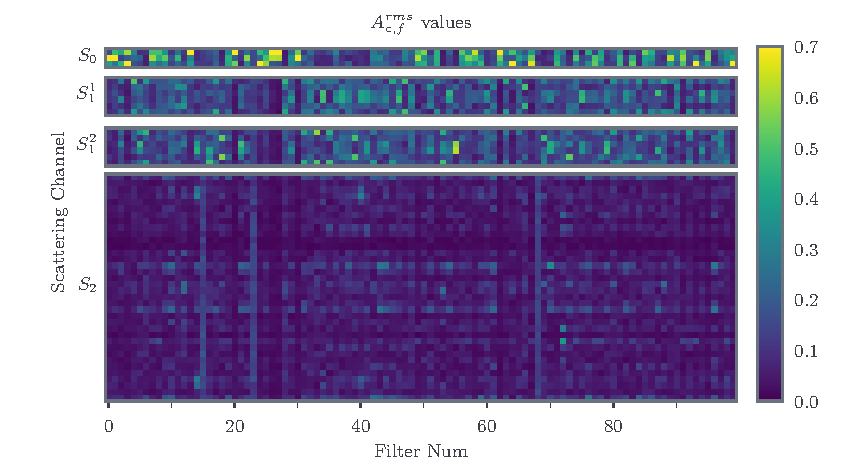
\includegraphics[width=15cm,height=8cm]{\imgpath/ti_conv1_weights.pdf}
  \mycaption{Channel weights for first learned layer}{A visualiztion of the
  matrix $A^{rms}$ from \eqref{eq:ch4:arms} for a network trained on Tiny
  ImageNet. The columns of the matrix all have
  unit norm and represent how much relative energy comes from each scattering
  output channel. Most of the filters are heavily dependent on $S_0$, many are 
  dependent on $S_1$ and only a few take information from $S_2$.}\label{fig:ch4:weights}
\end{figure}

\begin{figure}
  \vspace{0cm}
  \centering
  \subfloat[CIFAR-10]{\vspace{0cm}
    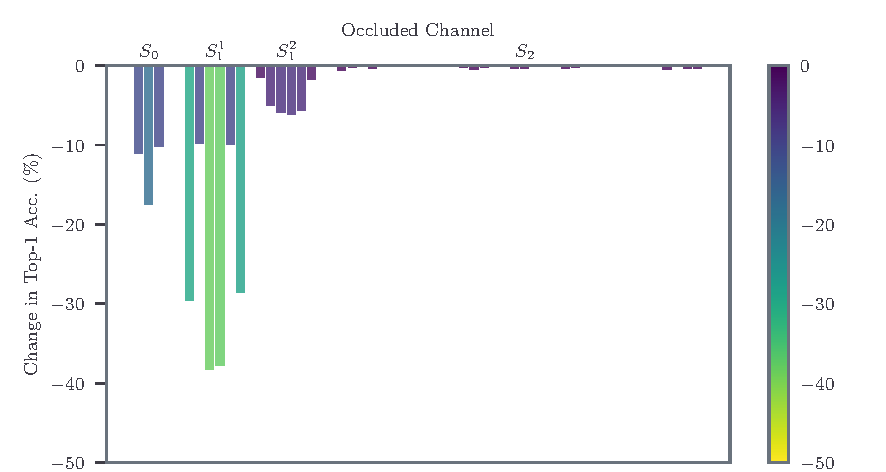
\includegraphics[width=15cm,height=8cm]{\imgpath/cifar10_occlusion_colour.pdf}
    \label{fig:ch4:cifar10_occlusion}
    }
    \\
  \subfloat[CIFAR-100]{
    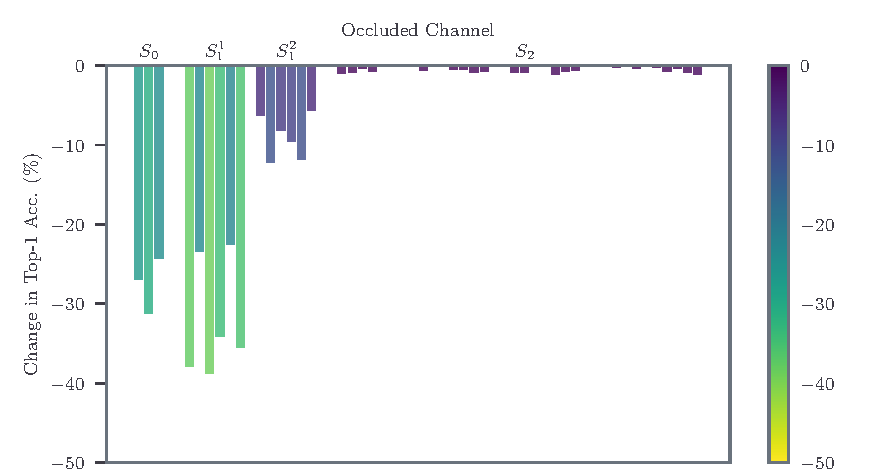
\includegraphics[width=15cm,height=8cm]{\imgpath/cifar100_occlusion_colour.pdf}
    \label{fig:ch4:cifar100_occlusion}
    }\vspace{-0.3cm}
  \mycaption{CIFAR changes in accuracy from channel occlusion}{Numbers
  reported are the drop in final classification accuracy when a channel is set
  to zero. The bars are coloured relative to their magnitude to aid seeing the
  differences for the $S_1$ coefficients. Unlike \autoref{fig:ch4:occlusion1}
  the $S_1^2$ coefficients are less important. CIFAR has a smaller image size than
  Tiny ImageNet so this is not surprising.}
  \label{fig:ch4:cifar_occlusion}
\end{figure}


